\subsection{File Cache Size}

\subsubsection{Estimation}

\subsubsection{Methodology}

\subsubsection{Results}

\subsubsection{Analysis}

\subsection{File Read Time}

In this section, we describe the time taken to read a file sequentially or randomly.

\subsubsection{Estimation}

Sequential access of a file is when we get the most out of the disk bandwidth. According to our vendor's specification, the maximum read throughput is 520MB/s. We are using a trick : we are not reading off a file that we have created. Rather, we are reading directly of from a disk partition, using a special file : \texttt{/dev/sda1}. In linux systems, \texttt{/dev/sda[x]} is the name of the special file representing disk partition \texttt{x}. There is no reason for a disk partition to be scattered across the disk (the way a user-generated file could be), therefore we can expect our disk access to be almost truly sequential (we still might have to fetch metadata on some other partition). As seen in class, we expect random access to be a lot slower than sequential access when accessing a file through disk. However, our machine uses a SSD, which are known to have much better seek times than traditional hard drives. 

\subsubsection{Methodology}

In order to ensure we are reading from disk and not from the file cache, we use the Linux flag \texttt{O\_DIRECT}. The \texttt{O\_DIRECT} flag can be specified when making the \texttt{open} system call. If used, it guarantees all read and write system calls on the opened file descriptor will fetch data from disk. We read from the \texttt{/dev/sda1} disk one MB at a time in a simple loop. We simulate different file sizes by setting a limit on the loop (called \texttt{total\_size}). When we reach the end of the loop we seek back to the beginning of the loop as follows : 

\begin{lstlisting}
if (total_read >= total_size) {
  retval = lseek64
     (fd, 0, SEEK_SET);
  total_read = 0;
  //...
\end{lstlisting}

where \texttt{total\_read} is the number of blocks read up to now in this iteration. To read blocks randomly, we also read directly from the disk partition. We use the \texttt{lseek} command which reads at an offset of a file descriptor, as follows:

\begin{lstlisting}
numblocks = SIZE_OF_FILE;
offset = (off64_t) numblocks *
  rand() / RAND_MAX;
retval = lseek64(fd, BLOCKSIZE 
  * offset, SEEK_SET);
\end{lstlisting}

where fd is the file seeked (in our case the disk partition), offset is the randomly chosen offset. \texttt{SEEK\_SET} is an option which tells the \texttt{lseek} command to start offsetting from the beginning of the file. Finally, we simulate files of varying size by changing the \texttt{numblocks} variable. Notice that we always access random locations within the files. To obtain the block size, we used a system command, \texttt{blockdev --getbsz /dev/sda1}; we found it was 4096. Notice we try to maximize bandwidth while reading truly randomly by seeking after each block read. If we read more than one block, than our read pattern would be partly sequential. If we read less, than we would not maximize our read bandwidth. Finally, in order to have good enough simulation we iterate continuously for 10 seconds and then measure the average time it takes to read one block into memory per millisecond.

\subsubsection{Results}

\begin{figure*}
 \centering
  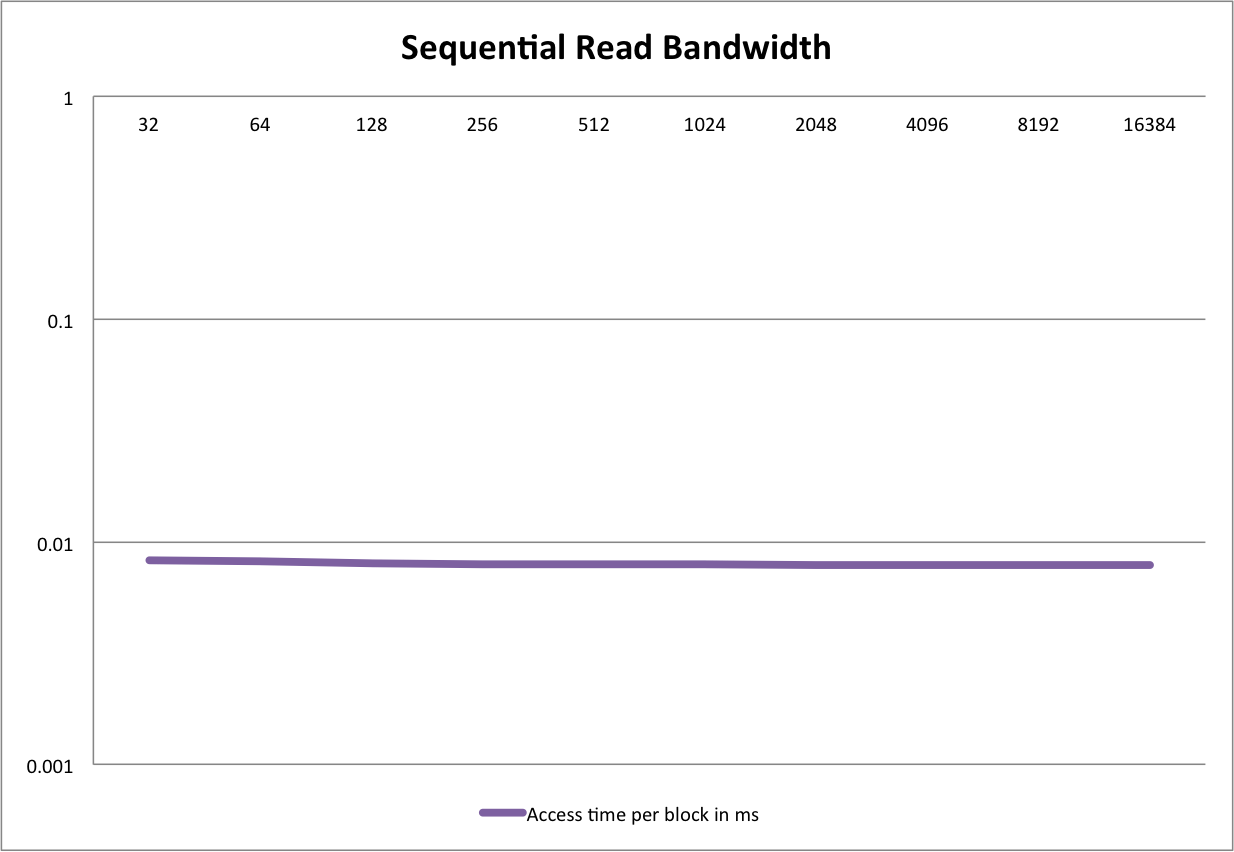
\includegraphics[width=0.85\textwidth]{image/sequential_read.png}
  \caption{Sequential Access Bandwidth}
 \label{fig:sequential}
\end{figure*}

\begin{figure*}
 \centering
  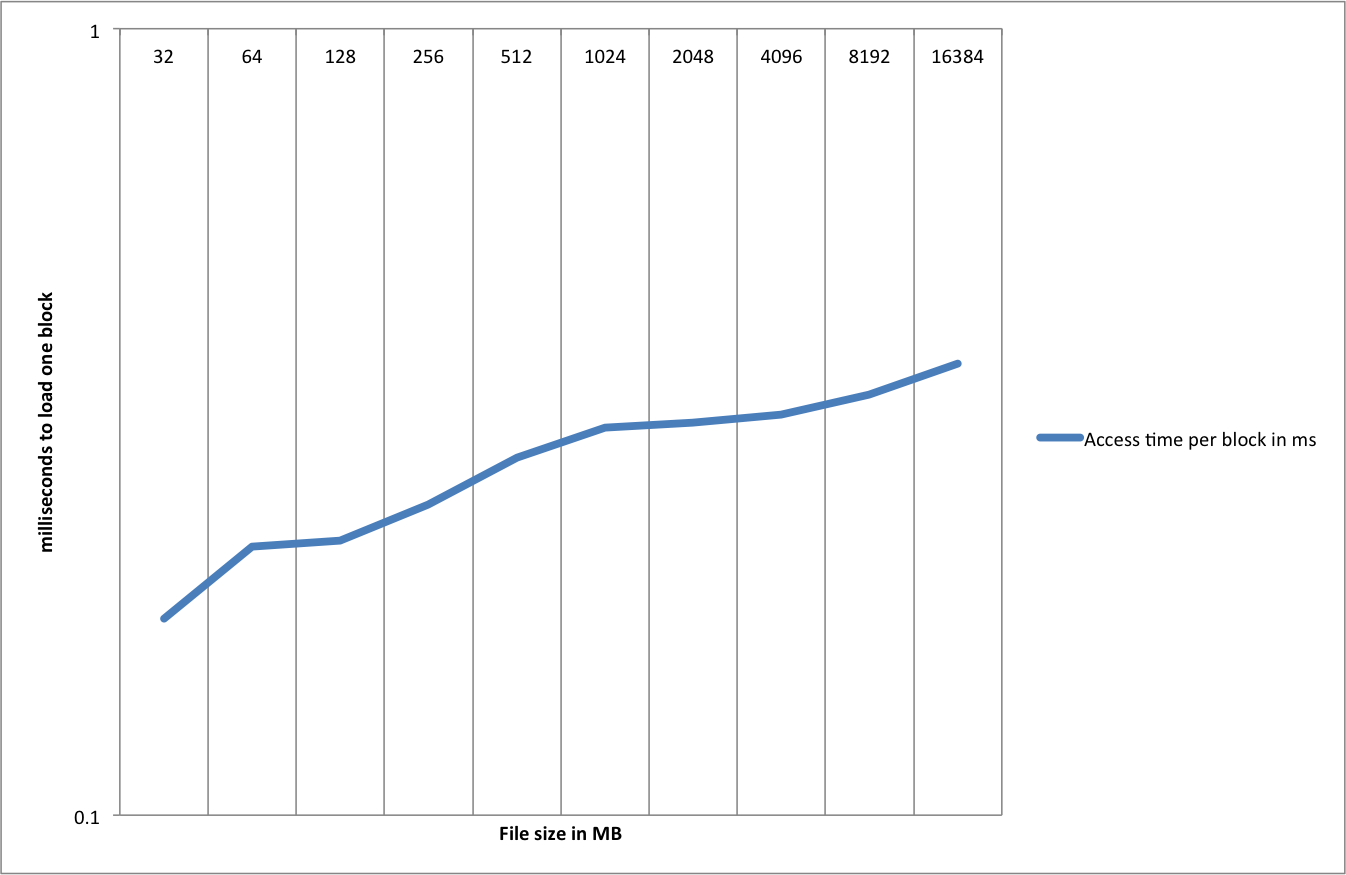
\includegraphics[width=0.85\textwidth]{image/random_read.png}
  \caption{Random Access Bandwidth}
 \label{fig:random}
\end{figure*}

Results can be seen on figures [\ref{fig:sequential}] and [\ref{fig:random}]. Both plots are using logarithmic scales for both axes.

\subsubsection{Analysis}

The sequential access time is extremely flat across file sizes. Indeed, we have no reason to expect the disk bandwidth to increase (or decrease) as the amount of data read grows bigger. On the other hand, we notice a slight increase in random access time as file size increases. There is no easy explanation for this on the operating system level. However, it is possible that an optimization exists within the SSD. Our SSD has a CPU, and might be doing some caching of its own which reduces random access times when files are smaller.

\subsection{Remote File Read Time}

\subsubsection{Estimation}

\subsubsection{Methodology}

\subsubsection{Results}

\subsubsection{Analysis}

\subsection{Contention}

\subsubsection{Estimation}

Disk access is a limited resource, and it would seem likely that in the case where multiple processes attempt to access the disk at the same time, performance would decrease. More specifically, if two processes would attempt to use the full bandwidth of the disk, than each one will end up with half the disk bandwidth (a linear coefficient of 2).

\subsubsection{Methodology}

To measure contention, we use instances of the random access file read profiler program (which we developed in 4.2). We create from one to twenty of those instances and run them concurrently. Each instance continuously queries the disk for 10 seconds before outputting statistics on its disk access time. Each instance reads a different file which is 256 MB long. 

\subsubsection{Results}

\begin{figure*}
 \centering
  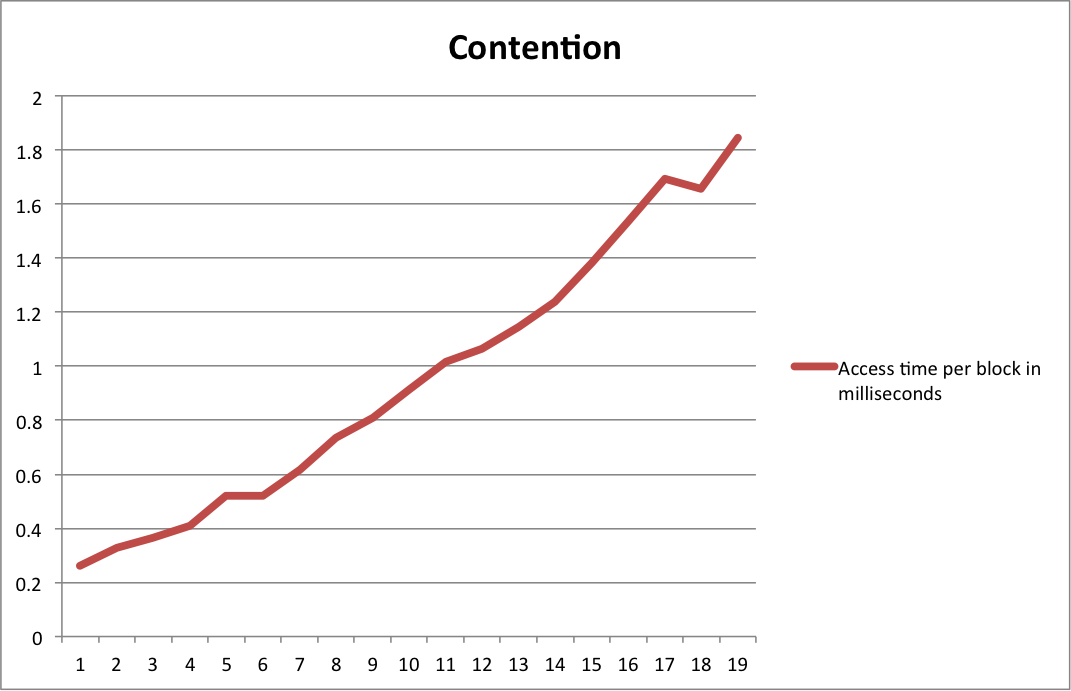
\includegraphics[width=0.85\textwidth]{image/contention.png}
  \caption{Sequential Access Bandwidth}
 \label{fig:contention}
\end{figure*}

Results for the contention experiment are reported on figure [\ref{fig:contention}].

\subsubsection{Analysis}

We notice that the access time per block increases linearly in the number of concurrent processes attempting to access the disk. However, it seems the disk is doing a little better than our estimate, in the sense that the linear coefficient which the disk seems to follow is closer to 1.5 than to 2. It is possible that some kind of optimization is done within the disk to serve the same data to multiple processes (in case where the SSD happens to fetch data for two clients). 